\chapter{Conception et architecture}

\usepackage{tikz}
\usetikzlibrary{shapes,arrows,positioning,fit,calc}

\section{Introduction}
Ce chapitre présente la conception détaillée et l'architecture technique 
de la fonctionnalité de recueil de feedbacks et de réclamations développée 
dans le cadre du stage chez Bewize. Avant d'aborder les aspects purement 
techniques, il est essentiel de comprendre le cadre méthodologique dans 
lequel ce projet a été conduit. En effet, le choix d'une méthodologie de 
gestion de projet adaptée est une condition indispensable au succès de tout 
projet informatique, particulièrement dans un contexte de stage en entreprise 
où les délais sont courts et les attentes précises.

Ce chapitre s'articule autour de quatre grands axes complémentaires et 
progressifs : premièrement, la méthodologie de gestion de projet adoptée 
(Agile et Scrum) qui a encadré l'ensemble du travail ; deuxièmement, 
l'architecture globale de la solution décrivant comment les différents 
composants s'articulent entre eux ; et troisièmement, la conception UML 
et les diagrammes modélisant le comportement et la structure du système.

%==========================================================
\section{Méthodologie de projet : Agile et Scrum}
%==========================================================

\subsection{Introduction à la méthodologie Agile}
Dans le domaine du développement logiciel moderne, le choix d'une 
méthodologie de gestion de projet adaptée est une condition indispensable 
au succès de tout projet informatique. Il existe deux grandes familles 
de méthodologies : les méthodes traditionnelles dites "en cascade" 
(Waterfall) et les méthodes agiles. Les méthodes traditionnelles suivent 
un processus séquentiel et rigide où chaque phase doit être entièrement 
terminée avant de passer à la suivante. Bien qu'elles offrent une structure 
claire, elles s'adaptent très difficilement aux changements de besoins 
en cours de projet, ce qui peut conduire à la livraison d'un produit 
qui ne correspond plus aux attentes réelles des utilisateurs.

Face à ces limitations, le mouvement Agile est apparu avec la publication 
du Manifeste Agile en février 2001, signé par dix-sept experts reconnus 
en développement logiciel. Ce manifeste définit quatre valeurs fondamentales :

\begin{itemize}
    \item \textbf{Les individus et leurs interactions} plutôt que les 
    processus et les outils : la communication directe entre les membres 
    de l'équipe est prioritaire sur le suivi rigide de procédures.
    
    \item \textbf{Des logiciels opérationnels} plutôt qu'une documentation 
    exhaustive : l'objectif est de livrer un produit fonctionnel apportant 
    une valeur concrète à l'utilisateur final.
    
    \item \textbf{La collaboration avec les clients} plutôt que la 
    négociation contractuelle : le représentant métier est impliqué tout 
    au long du projet.
    
    \item \textbf{L'adaptation au changement} plutôt que le suivi d'un 
    plan rigide : les méthodes agiles accueillent favorablement les 
    changements, même en cours de développement.
\end{itemize}

\begin{figure}[H]
    \centering
    
\includegraphics[width=0.8\textwidth]{Figures/agile.png}
    \caption{Le cycle de développement Agile}
    \label{fig:agile}
\end{figure}

\subsection{Le framework Scrum}
Parmi les nombreux frameworks agiles existants, Bewize a choisi d'adopter 
Scrum pour la gestion de ses projets de développement logiciel. Scrum est 
le framework agile le plus largement utilisé dans l'industrie du logiciel. 
Il a été formalisé par Ken Schwaber et Jeff Sutherland dans les années 1990.

Scrum organise le travail en cycles itératifs de durée fixe appelés Sprints, 
généralement d'une à quatre semaines. À la fin de chaque Sprint, l'équipe 
livre un incrément potentiellement déployable du produit.

\begin{figure}[H]
    \centering
    \includegraphics[width=0.88\textwidth]{Figures/scrum.png}
    \caption{Le framework Scrum — Vue d'ensemble}
    \label{fig:scrum}
\end{figure}

\subsection{Équipe de développement Scrum chez Bewize}
Une équipe Scrum est une unité cohésive de professionnels focalisés sur 
un seul objectif à la fois. Le Scrum Guide définit trois rôles distincts, 
chacun ayant des responsabilités précises et complémentaires.

\subsubsection{Le Product Owner — Product Manager Bewize}
Le Product Owner est responsable de maximiser la valeur du produit 
résultant du travail de l'équipe. Dans le cadre du projet Bewize, ce rôle 
est assuré par le Product Manager de l'entreprise :
\begin{itemize}
    \item Définir et communiquer clairement l'objectif du produit
    \item Créer, maintenir et prioriser le Product Backlog
    \item Valider les fonctionnalités livrées à chaque fin de Sprint
    \item Prendre les décisions finales concernant le périmètre du projet
\end{itemize}

\subsubsection{Le Scrum Master — Tech Lead Bewize}
Le Scrum Master est responsable du bon fonctionnement de Scrum au sein 
de l'équipe. Dans le projet Bewize, le Tech Lead assure ce rôle :
\begin{itemize}
    \item Coacher les membres de l'équipe dans l'application des pratiques Scrum
    \item Identifier et éliminer les obstacles qui bloquent la progression
    \item Faciliter tous les événements Scrum et assurer la revue de code
    \item Protéger l'équipe des interruptions externes non planifiées
\end{itemize}

\subsubsection{L'équipe de développement}
\begin{itemize}
    \item \textbf{Lamyaa Lamssaoui (stagiaire) :} développement du 
    formulaire WebView React JS et intégration dans l'application mobile
    \item \textbf{L'équipe de développement Bewize :} support technique, 
    développement back-end Spring Boot et intégration dans l'existant
\end{itemize}

\begin{figure}[H]
    \centering
    
\includegraphics[width=0.78\textwidth]{Figures/equipe_scrum.png}
    \caption{Les rôles au sein de l'équipe Scrum chez Bewize}
    \label{fig:equipe_scrum}
\end{figure}

\subsection{Avantages de la méthodologie Scrum}

\textbf{Livraison rapide et régulière de valeur :}
Scrum organise le travail en Sprints courts de deux semaines, permettant 
de livrer des fonctionnalités démontrables régulièrement.

\textbf{Flexibilité et capacité d'adaptation :}
Scrum permet d'intégrer les changements dans le prochain Sprint sans 
perturber l'ensemble du planning global du projet.

\textbf{Réduction significative des risques :}
En organisant des revues régulières, Scrum permet d'identifier et de 
résoudre les problèmes bien avant qu'ils ne deviennent critiques.

\textbf{Amélioration continue des pratiques :}
Les Sprint Retrospectives permettent à l'équipe d'identifier régulièrement 
les points à améliorer dans ses pratiques de travail.

\textbf{Communication et collaboration renforcées :}
Les rituels Scrum créent un cadre structuré favorisant une communication 
transparente entre tous les membres de l'équipe.

\begin{figure}[H]
    \centering
    
\includegraphics[width=0.82\textwidth]{Figures/avantages_scrum.png}
    \caption{Les avantages de la méthodologie Scrum}
    \label{fig:avantages_scrum}
\end{figure}

\subsection{Le Product Backlog}
Le Product Backlog est le premier artefact officiel de Scrum. Il s'agit 
d'une liste ordonnée et exhaustive de tout ce qui est nécessaire pour 
améliorer le produit. Chaque élément est exprimé sous forme de User 
Story suivant le format :

\begin{center}
\textit{"En tant que [rôle], je veux [fonctionnalité] afin de [bénéfice]."}
\end{center}

\begin{table}[H]
\centering
\renewcommand{\arraystretch}{1.8}
\begin{tabular}{|c|p{7.5cm}|p{1.8cm}|p{1.5cm}|}
\hline
\textbf{ID} & \textbf{User Story} & \textbf{Priorité} & \textbf{Points} \\
\hline
US01 & En tant qu'utilisateur mobile, je veux voir un bouton feedback 
dans l'application afin d'y accéder facilement & Haute & 3 \\
\hline
US02 & En tant qu'utilisateur mobile, je veux être redirigé vers une 
WebView afin de remplir un formulaire simple & Haute & 5 \\
\hline
US03 & En tant qu'utilisateur mobile, je veux choisir entre feedback 
et réclamation afin de qualifier mon retour & Haute & 2 \\
\hline
US04 & En tant qu'utilisateur mobile, je veux saisir mon message dans 
un formulaire intuitif afin de transmettre mon retour & Haute & 3 \\
\hline
US05 & En tant qu'utilisateur mobile, je veux une confirmation après 
l'envoi afin de savoir que mon retour a été pris en compte & Moyenne & 2 \\
\hline
US06 & En tant qu'agent Bewize, je veux consulter les feedbacks dans 
le dashboard afin de les analyser et traiter & Haute & 5 \\
\hline
US07 & En tant qu'agent Bewize, je veux filtrer les retours par type 
et statut afin de prioriser les réclamations urgentes & Moyenne & 3 \\
\hline
US08 & En tant qu'agent Bewize, je veux changer le statut d'une 
réclamation afin de suivre son traitement & Haute & 3 \\
\hline
US09 & En tant qu'agent Bewize, je veux des statistiques sur les 
retours afin d'analyser les tendances & Basse & 5 \\
\hline
\end{tabular}
\caption{Product Backlog du projet}
\label{tab:product_backlog}
\end{table}

\begin{figure}[H]
    \centering
    
\includegraphics[width=0.85\textwidth]{Figures/product_backlog.png}
    \caption{Représentation visuelle du Product Backlog}
    \label{fig:product_backlog}
\end{figure}

\subsection{Le Sprint Backlog}
Le Sprint Backlog est le deuxième artefact officiel de Scrum. Le projet 
a été organisé en trois Sprints principaux de deux semaines :

\textbf{Sprint 1 — Semaines 3 et 4 : Développement du formulaire WebView}

\begin{table}[H]
\centering
\renewcommand{\arraystretch}{1.5}
\begin{tabular}{|p{7cm}|p{2.5cm}|p{2cm}|}
\hline
\textbf{Tâche} & \textbf{Responsable} & \textbf{Statut} \\
\hline
Création du projet React JS pour la WebView & Lamyaa & Terminé \\
\hline
Développement du composant formulaire & Lamyaa & Terminé \\
\hline
Intégration du choix feedback ou réclamation & Lamyaa & Terminé \\
\hline
Validation des champs obligatoires & Lamyaa & Terminé \\
\hline
Création de l'endpoint POST /api/feedbacks & Équipe dev & Terminé \\
\hline
Connexion du formulaire à l'API Spring Boot & Lamyaa & Terminé \\
\hline
Affichage du message de confirmation & Lamyaa & Terminé \\
\hline
Tests unitaires et correction des bugs & Lamyaa & Terminé \\
\hline
\end{tabular}
\caption{Sprint Backlog — Sprint 1}
\label{tab:sprint1}
\end{table}

\textbf{Sprint 2 — Semaines 5 et 6 : Intégration mobile et back-end}

\begin{table}[H]
\centering
\renewcommand{\arraystretch}{1.5}
\begin{tabular}{|p{7cm}|p{2.5cm}|p{2cm}|}
\hline
\textbf{Tâche} & \textbf{Responsable} & \textbf{Statut} \\
\hline
Intégration du composant WebView dans React Native & Lamyaa & Terminé \\
\hline
Ajout du bouton feedback dans l'application mobile & Lamyaa & Terminé \\
\hline
Gestion de la navigation vers et depuis la WebView & Lamyaa & Terminé \\
\hline
Connexion de l'API Spring Boot à PostgreSQL & Équipe dev & Terminé \\
\hline
Tests d'intégration bout en bout & Lamyaa + Tech Lead & Terminé \\
\hline
Correction des bugs identifiés & Lamyaa & Terminé \\
\hline
Validation technique par le Tech Lead & Tech Lead & Terminé \\
\hline
\end{tabular}
\caption{Sprint Backlog — Sprint 2}
\label{tab:sprint2}
\end{table}

\textbf{Sprint 3 — Semaine 6 : Dashboard monitor}

\begin{table}[H]
\centering
\renewcommand{\arraystretch}{1.5}
\begin{tabular}{|p{7cm}|p{2.5cm}|p{2cm}|}
\hline
\textbf{Tâche} & \textbf{Responsable} & \textbf{Statut} \\
\hline
Développement de la page liste des retours & Lamyaa & Terminé \\
\hline
Développement de la page détail d'un retour & Lamyaa & Terminé \\
\hline
Implémentation du filtre par type et statut & Lamyaa & Terminé \\
\hline
Fonctionnalité de changement de statut & Lamyaa & Terminé \\
\hline
Création des endpoints GET côté Spring Boot & Équipe dev & Terminé \\
\hline
Tests fonctionnels complets du dashboard & Lamyaa & Terminé \\
\hline
Validation finale par le Product Manager & Product Manager & Terminé \\
\hline
\end{tabular}
\caption{Sprint Backlog — Sprint 3}
\label{tab:sprint3}
\end{table}

\begin{figure}[H]
    \centering
    
\includegraphics[width=0.88\textwidth]{Figures/sprint_backlog.png}
    \caption{Tableau Kanban du Sprint Backlog}
    \label{fig:sprint_backlog}
\end{figure}

\subsection{Planification des Sprints}

\begin{table}[H]
\centering
\renewcommand{\arraystretch}{1.8}
\begin{tabular}{|c|p{3cm}|p{4cm}|p{4cm}|}
\hline
\textbf{Semaine} & \textbf{Phase} & \textbf{Objectif} & \textbf{Livrable} \\
\hline
S1 & Immersion agile & Découverte de Bewize et formation Scrum & 
Compréhension du contexte \\
\hline
S2 & Sprint Planning & Cadrage et Product Backlog & 
Backlog priorisé \\
\hline
S3-S4 & Sprint 1 & Formulaire WebView & 
Formulaire connecté à l'API \\
\hline
S5-S6 & Sprint 2 & Intégration mobile & 
Application avec WebView intégrée \\
\hline
S6 & Sprint 3 & Dashboard monitor & 
Interface de consultation \\
\hline
S6 & Sprint Review & Démonstration & 
Validation Product Manager \\
\hline
S7-S8 & Clôture & Marketing digital & 
Présentation finale \\
\hline
\end{tabular}
\caption{Planification générale des Sprints}
\label{tab:planification}
\end{table}

\begin{figure}[H]
    \centering
    
\includegraphics[width=0.95\textwidth]{Figures/planning.png}
    \caption{Diagramme de Gantt — Planification du projet}
    \label{fig:planning}
\end{figure}

%==========================================================
\section{Architecture globale du système}
%==========================================================

\subsection{Vue d'ensemble}
L'architecture de la fonctionnalité développée s'articule autour de 
quatre composants principaux qui communiquent de manière cohérente et 
structurée. Cette architecture suit le modèle client-serveur classique, 
enrichi par l'utilisation d'une page WebView comme interface intermédiaire 
entre l'application mobile et le back-end.

\subsection{Les quatre composants}

\subsubsection{Application mobile Bewize (React Native)}
L'application mobile constitue le point d'entrée de la fonctionnalité. 
Elle est enrichie d'un bouton dédié permettant d'accéder au feedback 
ou à la réclamation, et intègre un composant WebView pour afficher le 
formulaire sans quitter l'application.

\subsubsection{Page WebView (React JS)}
Interface web légère affichée dans l'application mobile via le composant 
WebView. Elle contient le formulaire de saisie, valide les données et 
les envoie au back-end Spring Boot via des requêtes HTTP REST.

\subsubsection{Back-end Spring Boot}
Cœur du système exposant des APIs REST consommées par la WebView et le 
dashboard. Il gère la logique métier, valide les données et les persiste 
dans PostgreSQL.

\subsubsection{Dashboard Monitor (React JS)}
Interface web interne accessible uniquement par l'équipe Bewize pour 
consulter, filtrer et traiter les feedbacks et réclamations reçus.

\begin{figure}[H]
\centering
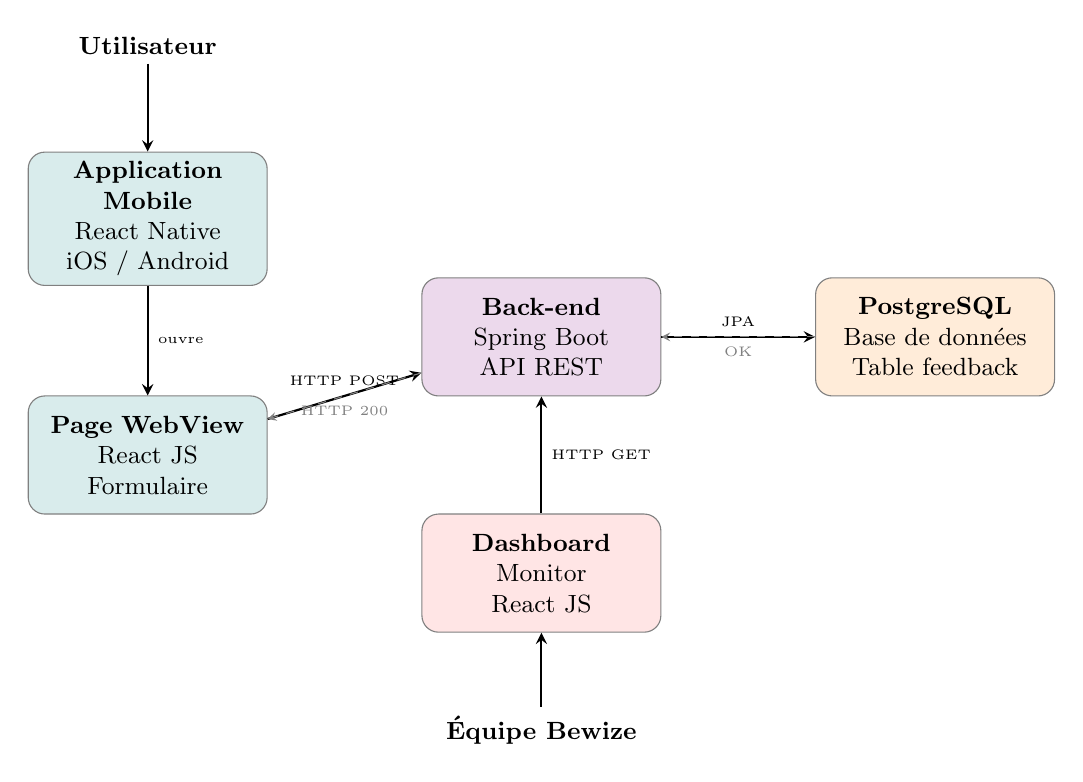
\begin{tikzpicture}[
    box/.style={rectangle, rounded corners=6pt, draw=black!50, 
                fill=gray!10, minimum width=3cm, minimum height=1.5cm,
                text width=2.8cm, align=center, font=\small},
    arrow/.style={->, >=stealth, thick},
    dasharrow/.style={->, >=stealth, dashed, gray}
]

% App Mobile
\node[box, fill=teal!15] (mobile) at (0,0) 
    {\textbf{Application Mobile}\\ React Native\\ iOS / Android};

% WebView
\node[box, fill=teal!15] (webview) at (0,-3) 
    {\textbf{Page WebView}\\ React JS\\ Formulaire};

% Backend
\node[box, fill=violet!15] (backend) at (5,-1.5) 
    {\textbf{Back-end}\\ Spring Boot\\ API REST};

% PostgreSQL
\node[box, fill=orange!15] (db) at (10,-1.5) 
    {\textbf{PostgreSQL}\\ Base de données\\ Table feedback};

% Dashboard
\node[box, fill=red!10] (dashboard) at (5,-4.5) 
    {\textbf{Dashboard}\\ Monitor\\ React JS};

% User
\node[font=\small] (user) at (0,2.2) {\textbf{Utilisateur}};
\draw[thick] (user) -- ++(0,-0.6);

% Team
\node[font=\small] (team) at (5,-6.5) {\textbf{Équipe Bewize}};

% Arrows
\draw[arrow] (mobile) -- (webview) node[midway, right, font=\tiny] {ouvre};
\draw[arrow] (webview) -- (backend) node[midway, above, font=\tiny] {HTTP POST};
\draw[dasharrow] (backend) -- (webview) node[midway, below, font=\tiny] {HTTP 200};
\draw[arrow] (backend) -- (db) node[midway, above, font=\tiny] {JPA};
\draw[dasharrow] (db) -- (backend) node[midway, below, font=\tiny] {OK};
\draw[arrow] (dashboard) -- (backend) node[midway, right, font=\tiny] {HTTP GET};
\draw[arrow] (team) -- (dashboard);
\draw[arrow] (user) -- (mobile);

\end{tikzpicture}
\caption{Architecture globale de la solution}
\label{fig:architecture}
\end{figure}

\subsection{Flux de données}
Le flux de données suit un chemin précis en neuf étapes :
\begin{enumerate}
    \item L'utilisateur clique sur le bouton feedback dans l'application mobile
    \item L'application ouvre le composant WebView
    \item La WebView charge et affiche le formulaire React JS
    \item L'utilisateur remplit et soumet le formulaire
    \item La WebView envoie une requête HTTP POST à l'API Spring Boot
    \item Le back-end valide et traite les données reçues
    \item Les données sont persistées dans PostgreSQL
    \item Le back-end retourne une réponse HTTP 200 à la WebView
    \item L'équipe consulte les données via le dashboard monitor
\end{enumerate}

%==========================================================
\section{Conception et Diagrammes}
%==========================================================

\subsection{Introduction}
La modélisation UML (Unified Modeling Language) est un standard 
international pour la modélisation des systèmes orientés objet. 
Dans ce projet, trois diagrammes complémentaires ont été réalisés 
pour modéliser la fonctionnalité développée.

\subsection{Diagramme de cas d'utilisation}
Le diagramme de cas d'utilisation représente les interactions entre 
les acteurs et le système, permettant de visualiser l'ensemble des 
fonctionnalités du point de vue des utilisateurs.

\textbf{Acteurs identifiés :}
\begin{itemize}
    \item \textbf{Utilisateur mobile :} utilisateur final qui soumet 
    des feedbacks ou réclamations via la WebView
    \item \textbf{Équipe interne Bewize :} membres qui consultent et 
    traitent les retours dans le dashboard monitor
\end{itemize}

\begin{figure}[H]
\centering
\begin{tikzpicture}[
    usecase/.style={ellipse, draw=black!50, fill=teal!10, 
                    minimum width=4cm, minimum height=0.8cm,
                    text width=3.8cm, align=center, font=\small},
    actor/.style={font=\small, align=center},
    arrow/.style={->, >=stealth}
]

% System boundary
\draw[dashed, rounded corners=8pt, draw=black!40] 
    (1.5,-0.5) rectangle (9.5,-8.5);
\node[font=\small\bfseries] at (5.5,-0.2) {Système Bewize};

% Use cases
\node[usecase] (uc1) at (5.5,-1.5) {Envoyer un feedback};
\node[usecase] (uc2) at (5.5,-3) {Envoyer une réclamation};
\node[usecase, fill=violet!10] (uc3) at (5.5,-4.8) {Consulter les retours};
\node[usecase, fill=violet!10] (uc4) at (5.5,-6.3) {Traiter une réclamation};
\node[usecase, fill=violet!10] (uc5) at (5.5,-7.8) {Filtrer les retours};

% Actor left: Utilisateur mobile
\node[actor] (user) at (-0.5,-2.2) {
    \begin{tikzpicture}[scale=0.5]
        \draw (0,0.6) circle (0.3);
        \draw (0,0.3) -- (0,-0.4);
        \draw (-0.4,-0.1) -- (0.4,-0.1);
        \draw (0,-0.4) -- (-0.3,-0.8);
        \draw (0,-0.4) -- (0.3,-0.8);
    \end{tikzpicture}\\[2pt]
    Utilisateur\\mobile
};

% Actor right: Equipe Bewize
\node[actor] (team) at (11,-6.3) {
    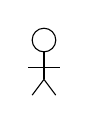
\begin{tikzpicture}[scale=0.5]
        \draw (0,0.6) circle (0.3);
        \draw (0,0.3) -- (0,-0.4);
        \draw (-0.4,-0.1) -- (0.4,-0.1);
        \draw (0,-0.4) -- (-0.3,-0.8);
        \draw (0,-0.4) -- (0.3,-0.8);
    \end{tikzpicture}\\[2pt]
    Équipe\\Bewize
};

% Connections user -> UC
\draw[arrow] (user) -- (uc1);
\draw[arrow] (user) -- (uc2);

% Connections team -> UC
\draw[arrow] (team) -- (uc3);
\draw[arrow] (team) -- (uc4);
\draw[arrow] (team) -- (uc5);

\end{tikzpicture}
\caption{Diagramme de cas d'utilisation}
\label{fig:use_case}
\end{figure}

\begin{table}[H]
\centering
\renewcommand{\arraystretch}{1.8}
\begin{tabular}{|c|p{4cm}|p{3cm}|p{5cm}|}
\hline
\textbf{ID} & \textbf{Cas d'utilisation} & \textbf{Acteur} & 
\textbf{Description} \\
\hline
UC01 & Envoyer un feedback & Utilisateur mobile & 
Soumettre un retour positif via la WebView \\
\hline
UC02 & Envoyer une réclamation & Utilisateur mobile & 
Signaler un problème ou une insatisfaction \\
\hline
UC03 & Consulter les retours & Équipe Bewize & 
Voir la liste dans le dashboard monitor \\
\hline
UC04 & Traiter une réclamation & Équipe Bewize & 
Changer le statut et prendre en charge \\
\hline
UC05 & Filtrer les retours & Équipe Bewize & 
Filtrer par type, date ou statut \\
\hline
\end{tabular}
\caption{Tableau des cas d'utilisation}
\label{tab:use_case}
\end{table}

\subsubsection{UC01 — Envoyer un feedback}
\begin{table}[H]
\centering
\renewcommand{\arraystretch}{1.5}
\begin{tabular}{|p{4cm}|p{9cm}|}
\hline
\textbf{Titre} & Envoyer un feedback \\
\hline
\textbf{Acteur principal} & Utilisateur mobile \\
\hline
\textbf{Précondition} & L'utilisateur est connecté à l'application Bewize \\
\hline
\textbf{Scénario nominal} & 
1. L'utilisateur clique sur le bouton feedback \newline
2. La WebView s'ouvre \newline
3. Il sélectionne "Feedback" \newline
4. Il saisit son message \newline
5. Il clique sur Envoyer \newline
6. Les données sont transmises à l'API \newline
7. Un message de confirmation est affiché \\
\hline
\textbf{Postcondition} & Le feedback est enregistré dans PostgreSQL \\
\hline
\textbf{Exception} & Erreur réseau : message d'erreur affiché \\
\hline
\end{tabular}
\caption{Description UC01 — Envoyer un feedback}
\end{table}

\subsubsection{UC02 — Envoyer une réclamation}
\begin{table}[H]
\centering
\renewcommand{\arraystretch}{1.5}
\begin{tabular}{|p{4cm}|p{9cm}|}
\hline
\textbf{Titre} & Envoyer une réclamation \\
\hline
\textbf{Acteur principal} & Utilisateur mobile \\
\hline
\textbf{Précondition} & L'utilisateur est connecté à l'application Bewize \\
\hline
\textbf{Scénario nominal} & 
1. L'utilisateur clique sur le bouton réclamation \newline
2. La WebView s'ouvre \newline
3. Il sélectionne "Réclamation" \newline
4. Il décrit son problème \newline
5. Il soumet le formulaire \newline
6. Les données sont transmises à l'API \newline
7. Un message de confirmation est affiché \\
\hline
\textbf{Postcondition} & La réclamation est visible dans le dashboard \\
\hline
\textbf{Exception} & Champs vides : message de validation affiché \\
\hline
\end{tabular}
\caption{Description UC02 — Envoyer une réclamation}
\end{table}

\subsubsection{UC03 — Consulter et traiter les retours}
\begin{table}[H]
\centering
\renewcommand{\arraystretch}{1.5}
\begin{tabular}{|p{4cm}|p{9cm}|}
\hline
\textbf{Titre} & Consulter et traiter les retours \\
\hline
\textbf{Acteur principal} & Équipe interne Bewize \\
\hline
\textbf{Précondition} & L'agent est authentifié sur le dashboard \\
\hline
\textbf{Scénario nominal} & 
1. L'agent accède au dashboard monitor \newline
2. Il consulte la liste des retours \newline
3. Il filtre par type ou statut \newline
4. Il clique sur un retour pour voir le détail \newline
5. Il change le statut en "En cours" puis "Traité" \\
\hline
\textbf{Postcondition} & La réclamation est marquée comme traitée \\
\hline
\textbf{Exception} & Aucun retour : message informatif affiché \\
\hline
\end{tabular}
\caption{Description UC03 — Consulter et traiter}
\end{table}

\subsection{Diagramme de séquence}
Le diagramme de séquence illustre le déroulement temporel des interactions 
entre les composants lors de l'envoi d'un feedback ou d'une réclamation.

\begin{figure}[H]
\centering
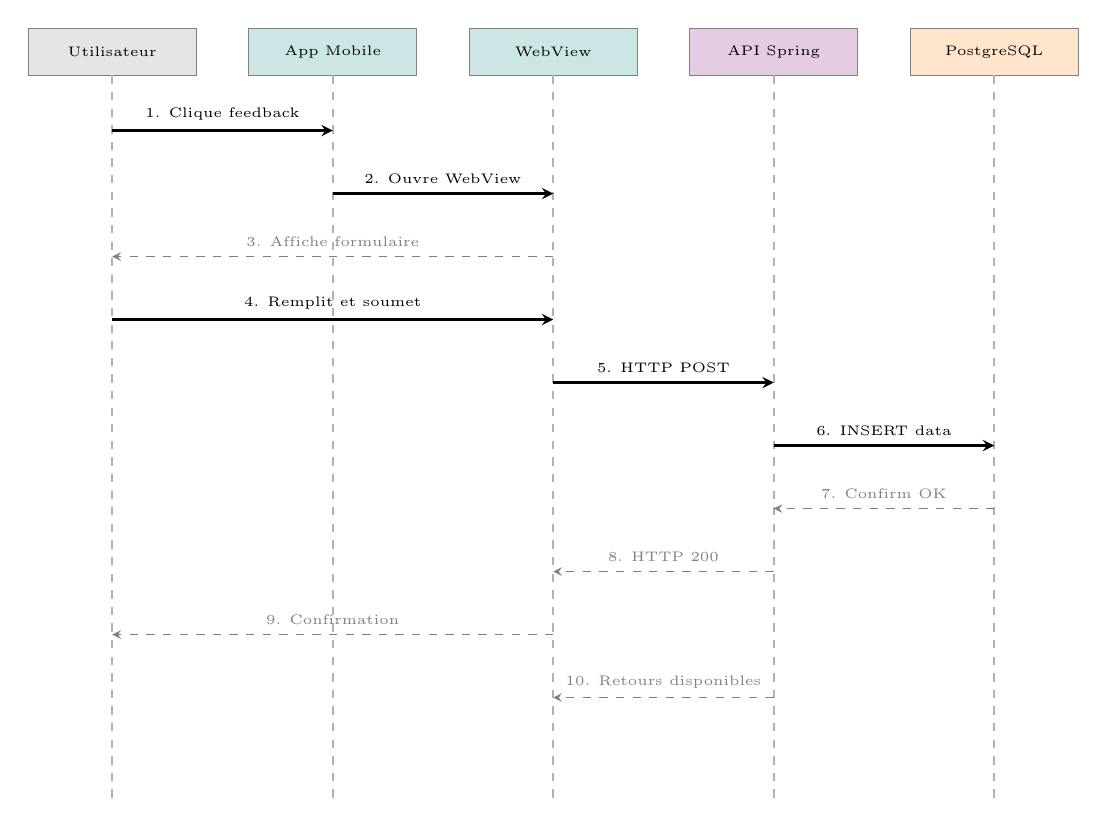
\begin{tikzpicture}[
    lifeline/.style={draw=black!30, dashed, thick},
    box/.style={rectangle, draw=black!50, fill=gray!15, 
                minimum width=2cm, minimum height=0.6cm,
                text width=1.9cm, align=center, font=\tiny},
    msg/.style={->, >=stealth, thick},
    ret/.style={->, >=stealth, dashed, gray},
    label/.style={font=\tiny, above}
]

% Header boxes
\node[box, fill=gray!20]    (u)  at (0,0)    {Utilisateur};
\node[box, fill=teal!20]    (m)  at (2.8,0)  {App Mobile};
\node[box, fill=teal!20]    (w)  at (5.6,0)  {WebView};
\node[box, fill=violet!20]  (a)  at (8.4,0)  {API Spring};
\node[box, fill=orange!20]  (db) at (11.2,0) {PostgreSQL};

% Lifelines
\draw[lifeline] (0,-0.3)   -- (0,-9.5);
\draw[lifeline] (2.8,-0.3) -- (2.8,-9.5);
\draw[lifeline] (5.6,-0.3) -- (5.6,-9.5);
\draw[lifeline] (8.4,-0.3) -- (8.4,-9.5);
\draw[lifeline] (11.2,-0.3)-- (11.2,-9.5);

% Messages
\draw[msg] (0,-1)    -- (2.8,-1)    node[label, midway] {1. Clique feedback};
\draw[msg] (2.8,-1.8)-- (5.6,-1.8)  node[label, midway] {2. Ouvre WebView};
\draw[ret] (5.6,-2.6)-- (0,-2.6)    node[label, midway] {3. Affiche formulaire};
\draw[msg] (0,-3.4)  -- (5.6,-3.4)  node[label, midway] {4. Remplit et soumet};
\draw[msg] (5.6,-4.2)-- (8.4,-4.2)  node[label, midway] {5. HTTP POST};
\draw[msg] (8.4,-5)  -- (11.2,-5)   node[label, midway] {6. INSERT data};
\draw[ret] (11.2,-5.8)--(8.4,-5.8)  node[label, midway] {7. Confirm OK};
\draw[ret] (8.4,-6.6)-- (5.6,-6.6)  node[label, midway] {8. HTTP 200};
\draw[ret] (5.6,-7.4)-- (0,-7.4)    node[label, midway] {9. Confirmation};
\draw[ret] (8.4,-8.2)-- (5.6,-8.2)  node[label, midway] {10. Retours disponibles};

\end{tikzpicture}
\caption{Diagramme de séquence — Envoi d'un feedback ou réclamation}
\label{fig:sequence}
\end{figure}

Le scénario se déroule en dix étapes :
\begin{enumerate}
    \item L'utilisateur clique sur le bouton dans l'application React Native
    \item L'application ouvre le composant WebView
    \item La WebView charge le formulaire React JS
    \item L'utilisateur remplit et soumet le formulaire
    \item La WebView envoie une requête HTTP POST à l'API Spring Boot
    \item Le back-end valide les données reçues
    \item Les données sont persistées dans PostgreSQL
    \item PostgreSQL confirme l'enregistrement
    \item Le back-end retourne HTTP 200 à la WebView
    \item La WebView affiche le message de confirmation
\end{enumerate}

\subsection{Diagramme de classes}
Le diagramme de classes représente la structure statique du système. 
L'architecture back-end suit le pattern en couches de Spring Boot.

\begin{figure}[H]
\centering
\begin{tikzpicture}[
    class/.style={rectangle, draw=black!50, fill=white,
                  minimum width=3.5cm, font=\tiny},
    header/.style={rectangle, draw=black!50, fill=gray!20,
                   minimum width=3.5cm, minimum height=0.5cm,
                   align=center, font=\tiny\bfseries},
    arrow/.style={->, >=stealth, thick},
    dasharrow/.style={->, >=stealth, dashed}
]
% FeedbackController
\node[header, fill=violet!20] (ch) at (0,0) {FeedbackController};
\node[class, below=0pt of ch, align=left, text width=3.3cm, 
      minimum height=1.4cm] (cb) 
    {- feedbackService\\
     \hline\\
     + createFeedback()\\
     + getAllFeedbacks()\\
     + updateStatut()};

% FeedbackService
\node[header, fill=teal!20] (sh) at (4.5,0) {FeedbackService};
\node[class, below=0pt of sh, align=left, text width=3.3cm,
      minimum height=1.4cm] (sb) 
    {- feedbackRepo\\
     \hline\\
     + save(feedback)\\
     + findAll()\\
     + updateStatut()\\
     + getStats()};

% FeedbackRepository
\node[header, fill=orange!20] (rh) at (9,0) {FeedbackRepository};
\node[class, below=0pt of rh, align=left, text width=3.3cm,
      minimum height=1.4cm] (rb) 
    {\textit{«interface»}\\
     \hline\\
     + findByType()\\
     + findByStatut()};

% Feedback Entity
\node[header, fill=red!10] (fh) at (4.5,-4.5) {Feedback};
\node[class, below=0pt of fh, align=left, text width=3.3cm,
      minimum height=1.8cm] (fb) 
    {- id: Long\\
     - type: String\\
     - message: String\\
     - dateEnvoi: DateTime\\
     - statut: String\\
     - utilisateurId: Long\\
     \hline\\
     + getters()\\
     + setters()};

% Utilisateur Entity
\node[header, fill=gray!20] (uh) at (9,-4.5) {Utilisateur};
\node[class, below=0pt of uh, align=left, text width=3.3cm,
      minimum height=1.2cm] (ubb) 
    {- id: Long\\
     - nom: String\\
     - email: String\\
     \hline\\
     + getters()\\
     + setters()};
% Arrows
\draw[arrow] (cb) -- (sb) node[midway, above, font=\tiny] {uses};
\draw[arrow] (sb) -- (rb) node[midway, above, font=\tiny] {uses};
\draw[arrow] (sb) -- (fh) node[midway, right, font=\tiny] {manages};
\draw[dasharrow] (rb) -- (fh) node[midway, left, font=\tiny] {};
\draw[arrow] (fb) -- (ubb) node[midway, above, font=\tiny] {belongs to};

\end{tikzpicture}
\caption{Diagramme de classes}
\label{fig:classes}
\end{figure}

Les classes principales sont :
\begin{itemize}
    \item \textbf{Feedback (Entity) :} classe centrale avec les attributs 
    id, type, message, dateEnvoi, statut et utilisateurId
    \item \textbf{FeedbackController :} expose les endpoints REST API 
    et délègue au FeedbackService
    \item \textbf{FeedbackService :} implémente la logique métier et 
    coordonne entre le contrôleur et le repository
    \item \textbf{FeedbackRepository :} interface JPA gérant la 
    persistance dans PostgreSQL
    \item \textbf{Utilisateur :} représente l'utilisateur de 
    l'application mobile
\end{itemize}

\subsection{Conception de la base de données}

\begin{table}[H]
\centering
\renewcommand{\arraystretch}{1.5}
\begin{tabular}{|p{3cm}|p{3cm}|p{2.5cm}|p{4.5cm}|}
\hline
\textbf{Champ} & \textbf{Type} & \textbf{Contrainte} & \textbf{Description} \\
\hline
id & BIGINT & PRIMARY KEY & Identifiant unique auto-incrémenté \\
\hline
type & VARCHAR(20) & NOT NULL & FEEDBACK ou RECLAMATION \\
\hline
message & TEXT & NOT NULL & Contenu du message \\
\hline
date\_envoi & DATETIME & NOT NULL & Date et heure d'envoi \\
\hline
statut & VARCHAR(20) & NOT NULL & NOUVEAU, EN\_COURS, TRAITE \\
\hline
utilisateur\_id & BIGINT & FOREIGN KEY & Référence à l'utilisateur \\
\hline
\end{tabular}
\caption{Structure de la table feedback}
\label{tab:bdd}
\end{table}

\subsection{Conception de l'API REST}

\begin{table}[H]
\centering
\renewcommand{\arraystretch}{1.5}
\begin{tabular}{|p{1.8cm}|p{5cm}|p{2cm}|p{4cm}|}
\hline
\textbf{Méthode} & \textbf{Endpoint} & \textbf{Accès} & \textbf{Description} \\
\hline
POST & /api/feedbacks & WebView & Soumettre un retour \\
\hline
GET & /api/feedbacks & Dashboard & Liste de tous les retours \\
\hline
GET & /api/feedbacks/\{id\} & Dashboard & Détail d'un retour \\
\hline
PUT & /api/feedbacks/\{id\}/statut & Dashboard & Mettre à jour le statut \\
\hline
GET & /api/feedbacks/stats & Dashboard & Statistiques des retours \\
\hline
\end{tabular}
\caption{Endpoints REST API}
\label{tab:api}
\end{table}

%==========================================================
\section{Conclusion}
%==========================================================

Ce chapitre a présenté de manière complète et structurée l'ensemble 
des aspects méthodologiques, architecturaux et conceptuels du projet 
développé chez Bewize.

La méthodologie Agile Scrum, avec ses trois Sprints bien définis, 
ses artefacts (Product Backlog et Sprint Backlog) et ses événements 
(Sprint Planning, Daily Scrum, Sprint Review), a permis d'organiser 
le travail de manière itérative et efficace.

L'architecture en quatre composants (application mobile, WebView, 
back-end et dashboard) garantit une séparation claire des responsabilités. 
Les diagrammes UML réalisés — cas d'utilisation, séquence et classes — 
constituent une base solide pour la phase d'implémentation détaillée 
dans le chapitre suivant.